\section{Experiments}
\label{sec:result}

All numbers are 5-fold cross-validation means on the validation (``test'') split of
the \texttt{price} target (USD). We first compare every model across the four
location-encoding variants (Tables~\ref{tab:single}--\ref{tab:ensemble}), then
report full metrics for the headline configurations (Table~\ref{tab:headline}).
The naive baseline throughout is \texttt{rf}/\texttt{cat}.

% ============================================================
\subsection{Model $\times$ Encoding Comparison}
% ============================================================

\begin{table}[h]
\centering
\caption{Single models --- validation Adjusted $R^2$ (mean $\pm$ std) by encoding variant.}
\label{tab:single}
\begin{tabular}{lcccc}
\toprule
\textbf{Model} & \texttt{cat} & \texttt{coord\_only} & \texttt{tgt\_only} & \texttt{tgt} \\
\midrule
MLP             & $0.533 \pm 0.082$ & $0.680 \pm 0.069$ & $0.717 \pm 0.053$ & $0.724 \pm 0.045$ \\
DT              & $0.443 \pm 0.085$ & $0.608 \pm 0.054$ & $0.645 \pm 0.061$ & $0.633 \pm 0.072$ \\
RF              & $0.667 \pm 0.047$ & $0.753 \pm 0.046$ & $0.743 \pm 0.048$ & $0.754 \pm 0.048$ \\
mGBDT (XGBoost) & $0.665 \pm 0.044$ & $0.744 \pm 0.045$ & $0.753 \pm 0.041$ & $\mathbf{0.765 \pm 0.043}$ \\
\bottomrule
\end{tabular}
\end{table}

\begin{table}[h]
\centering
\caption{Stacking ensembles --- validation Adjusted $R^2$ (mean $\pm$ std) by encoding variant.}
\label{tab:ensemble}
\begin{tabular}{lcccc}
\toprule
\textbf{Model} & \texttt{cat} & \texttt{coord\_only} & \texttt{tgt\_only} & \texttt{tgt} \\
\midrule
MLP             & $0.581 \pm 0.047$ & $0.698 \pm 0.044$ & $0.749 \pm 0.047$ & $0.779 \pm 0.050$ \\
DT              & $0.598 \pm 0.035$ & $0.718 \pm 0.050$ & $0.716 \pm 0.054$ & $0.713 \pm 0.053$ \\
RF              & $0.739 \pm 0.053$ & $\mathbf{0.794 \pm 0.048}$ & $0.770 \pm 0.053$ & $0.782 \pm 0.053$ \\
mGBDT (XGBoost) & $0.698 \pm 0.052$ & $0.753 \pm 0.049$ & $0.762 \pm 0.058$ & $0.771 \pm 0.051$ \\
\bottomrule
\end{tabular}
\end{table}

Two trends are immediate. First, moving from the naive \texttt{cat} encoding to any
coordinate- or target-aware variant lifts every model substantially: the baseline
RF rises from $0.667$ (\texttt{cat}) to $0.754$ (\texttt{tgt}), and the worst cell,
DT/\texttt{cat} at $0.443$, is far below any encoded configuration.
Figure~\ref{fig:rf_variants} shows this effect for RF in isolation.
Second, stacking the price and price-per-sqft models adds a further gain for the
stronger models---most notably RF, whose best ensemble (\texttt{coord\_only},
$0.794$) exceeds its best single model ($0.754$) and is the top configuration
overall.

\begin{figure}[h]
\centering
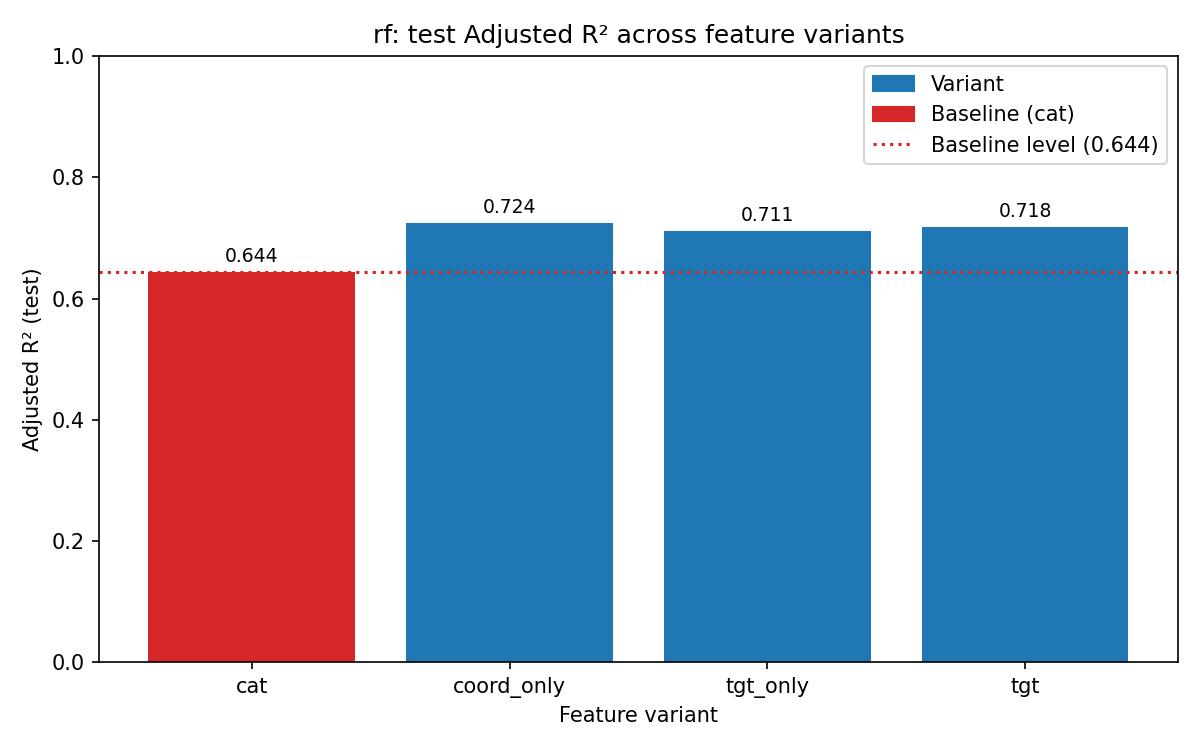
\includegraphics[width=0.62\textwidth]{results/rf_variant_comparison_test.png}
\caption{Random Forest validation Adjusted $R^2$ across the four encoding variants.
Every encoded variant beats the naive \texttt{cat} baseline (dotted line).}
\label{fig:rf_variants}
\end{figure}

% ============================================================
\subsection{Headline Configurations}
% ============================================================

\begin{table}[h]
\centering
\caption{Full validation metrics for headline configurations (\texttt{price} target).
RMSE/MAE in thousand USD; $R^2$ and Adj.\ $R^2$ are across-fold means.}
\label{tab:headline}
\begin{tabular}{llccccc}
\toprule
\textbf{Configuration} & & \textbf{RMSE} & \textbf{MAE} & \textbf{MAPE (\%)} & \textbf{$R^2$} & \textbf{Adj.\ $R^2$} \\
\midrule
\texttt{rf} / \texttt{cat}            & (baseline)    & 197.1 & 112.1 & 22.85 & 0.673 & 0.667 \\
\texttt{rf} / \texttt{tgt}            & (single)      & 168.4 &  88.5 & 17.67 & 0.759 & 0.754 \\
mGBDT(XGBoost) / \texttt{tgt}         & (best single) & 164.9 &  90.4 & 18.58 & 0.770 & 0.765 \\
ensemble \texttt{rf} / \texttt{tgt}   & (stacked)     & 158.0 &  84.8 & 17.24 & 0.787 & 0.782 \\
ensemble \texttt{rf} / \texttt{coord\_only} & (best)  & \textbf{154.1} & \textbf{84.2} & 17.38 & \textbf{0.798} & \textbf{0.794} \\
\bottomrule
\end{tabular}
\end{table}

Relative to the baseline, the best configuration cuts RMSE from $197.1$k to $154.1$k
(a $22\%$ reduction) and raises Adjusted $R^2$ from $0.667$ to $0.794$.
Figure~\ref{fig:top7} ranks the top-7 (model, variant) pairs against the
baseline, among single models (left) and including the stacking ensembles (right).

\begin{figure}[h]
\centering
\begin{minipage}{0.49\textwidth}
\centering
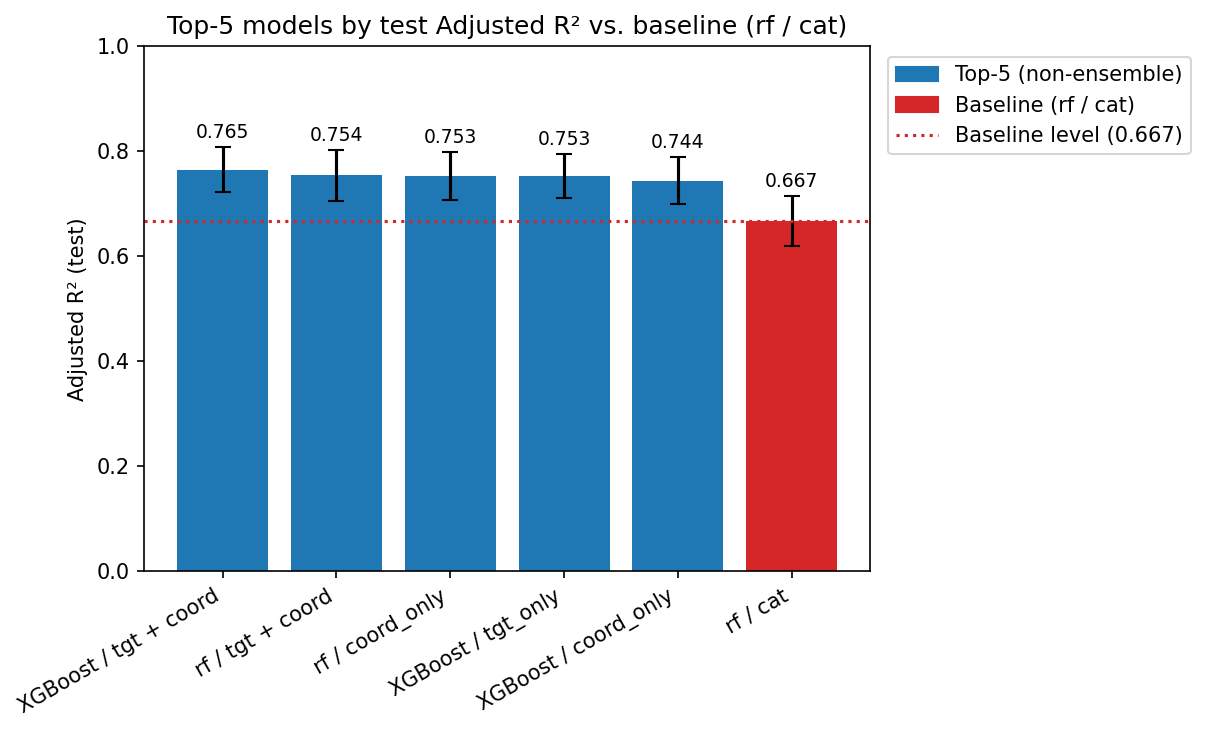
\includegraphics[width=\textwidth]{results/top5_adjusted_r2_test_no_ensemble.png}
\end{minipage}\hfill
\begin{minipage}{0.49\textwidth}
\centering
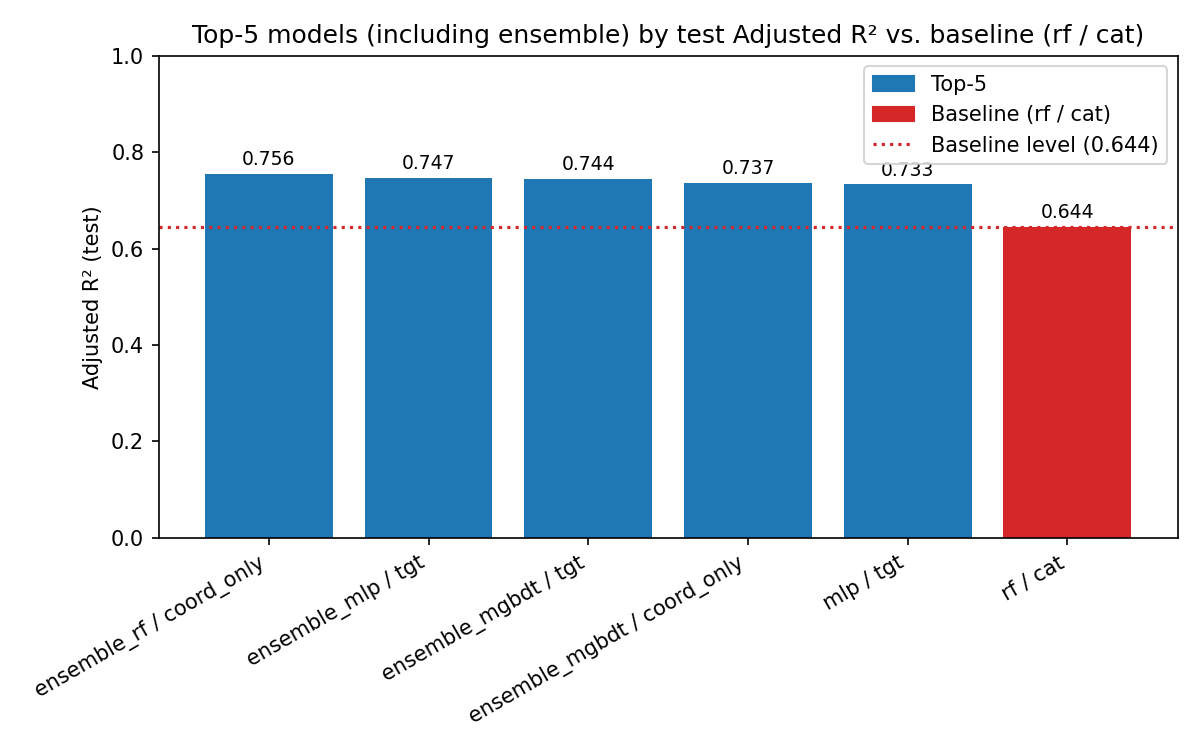
\includegraphics[width=\textwidth]{results/top5_adjusted_r2_test.png}
\end{minipage}
\caption{Top-7 configurations by validation Adjusted $R^2$ vs.\ the
\texttt{rf}/\texttt{cat} baseline: single models (left) and including stacking
ensembles (right). The best, ensemble \texttt{rf}/\texttt{coord\_only}, reaches
$0.794$.}
\label{fig:top7}
\end{figure}

% ============================================================
\subsection{Discussion}
% ============================================================

\textbf{Encoding helps, but its effect is model-dependent.}
Coordinate and target encoding both beat naive categorical encoding across the
board, confirming that the location fields carry real, recoverable signal. Which
of the two wins, however, depends on the model and is not decisive: for RF the
\texttt{coord\_only} and \texttt{tgt} variants are within noise of each other, and
combining both (\texttt{tgt}) is not uniformly best. We attribute the ambiguity to
geography---house values respond to nearby oceans, mountains, and roads that
neither a smoothed category mean nor a raw coordinate fully captures.

\textbf{Stacking recovers signal beyond size.}
The price / price-per-sqft ensemble improves the stronger models because dividing by
living area regularizes the size-dominated, outlier-heavy price target. The best
ensemble (\texttt{rf}/\texttt{coord\_only}, $0.794$) beats both the naive baseline
($0.667$) and the best standard single boosting model (mGBDT/XGBoost on \texttt{tgt},
$0.765$), supporting the hypothesis that deeper relationships emerge once
domain-aware preprocessing offsets the dominance of \texttt{sqft\_living}.

\textbf{mGBDT did not justify its depth.}
A two-layer mGBDT was outperformed by the single-layer (plain XGBoost) configuration:
the first XGBoost layer already had sufficient expressive power, and the second layer
fit noise rather than additional structure. Consistent with this, the single-layer
``mGBDT (XGBoost)'' is the best \emph{single} model but does not dominate the tuned
ensembles. We therefore adopt XGBoost as the final boosting model and conclude that
this dataset lacks the hierarchical complexity that mGBDT is designed to exploit.
